%-------------------------------------------------------------------------------
%
%     CHARGEMENT DES EXTENSIONS
%
%-------------------------------------------------------------------------------
\documentclass[11pt,fleqn]{report}
\usepackage{GarmirKhatch}
\usepackage[utf8]{inputenc}
%-------------------------------------------------------------------------------
%     Informations spécifiques au document
%-------------------------------------------------------------------------------
\ZTitle{Système de gestion des transports}
\ZSubject{Authentification et contrôle d'accès}
\ZVersion{1.0}
\ZDate{\today}
\ZAuthor{\Balde,\\\Cadon,\\\Gairoard,\\\Julien,\\\Lericolais,\\\Mezelle,\\\Pachy,\\\SuangaWeto,\\\Toure}
%-------------------------------------------------------------------------------
%     Contenu
%-------------------------------------------------------------------------------


\begin{document}
    
\ZMakeCover

\ZMakeInformations{
	    % Historique des modifications
	    % Version & Date & Auteur(s) & Modification(s)
	    0.1 & 2014-03-25 & \Mezelle  & Création \\
	    \midrule
	    0.1 & 2014-03-26 & \SuangaWeto & mis à jour \\
	    \midrule
    }{
	    % Historique des approbations
	    % Version & Date & Approbateur(s)
	    \ZVersion & - & - \\
    }{
	    % Historique des validations
	    % Version & Date & Responsable(s)
	    0.1 & - & - \\
    }

\ZMakeTableOfContents

\chapter{Introduction}
Dans le cadre de la mission confiée par Garmir Katch nous avons pour tâche de mettre en place un module d’authentification et de contrôle d’accès à intégrer à la solution finale. Pour cela nous nous basons sur une base de données d’annuaire afin de regrouper les informations sur les utilisateurs de la société (informations personnelles, droits, groupes).

Un annuaire est prévu pour être plus sollicité en lecture qu'en écriture. Cela signifie qu'un annuaire est conçu pour être plus souvent consulté que mis à jour. Dans notre cas les utilisateurs auront d’avantage besoin d’accéder à la base de données en lecture plutôt que pour y modifier des champs (d’où le choix d’une base de données d’annuaire plutôt qu’une relationnelle).

Cet annuaire est géré par le protocole LDAP (Lightweight Directory Acces Protocol).
\chapter{Pourquoi LDAP ?}
Le protocole LDAP présente plusieurs avantages liés aux exigences de l’utilisation d’un annuaire plutôt qu’une base de données relationnelle :
\begin{itemize}
\item Les annuaires doivent être compacts et reposer sur un protocole réseau léger : comme son nom l’indique c’est un protocole allégé pour accéder aux annuaires.
\item Un serveur d'annuaire doit comporter des mécanismes permettant de coopérer, c'est-à-dire d'étendre la recherche sur des serveurs tiers si jamais aucun enregistrement n'est trouvé : le protocole LDAP dispose d’un mécanisme de référencement (referral).
\item Un annuaire doit être capable de gérer l'authentification des utilisateurs ainsi que les droits de ceux-ci pour la consultation ou la modification de données : LDAP fourni une méthode d’authentification (bind).
\item Possibilité de sécuriser la connexion en TLS via un port spécifique utilisant le protocole LDAPS.
\item Répartition possible de l’annuaire sur plusieurs points d’accès via un service de réplication fourni par LDAP.
\item Ce même service permet une haute disponibilité des serveurs.
\end{itemize}
Ces fonctionnalités nous permettent de répondre à la demande d'optimisation des flux (protocole léger), à la sécurité (disponibilité, confidentialité)


L'intérêt principal de LDAP est la normalisation de l'authentification. Il est facile de programmer un module d'authentification utilisant LDAP à partir d'un langage possédant une API LDAP.
\chapter{Structure de l'annuaire}
\begin{figure}[htbp]
	\centering
	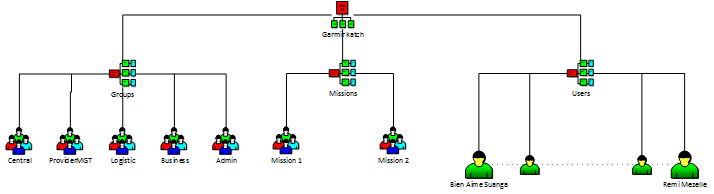
\includegraphics[scale=0.9]{Images/SchemaLDAP.png}
	\caption{Schéma de l'annuaire LDAP mis en place}
	\label{SchemaLDAP}
\end{figure}
L’annuaire est organisé en trois parties :
\begin{itemize}
\item la première recense toutes les personnes de la société et leurs droits,
\item la deuxième concerne les différents groupes d’utilisateurs et les droits de chaque groupe,
\item la troisième permet de rassembler les personnes présentes sur chaque mission.
\end{itemize}

Chaque utilisateur dispose d’un identifiant unique (uid) et d’un mot de passe (userPassword) et aussi différents champs représentant ses droits. Le mot de passe d’un utilisateur est stocké en haché SSHA. Enfin, il est possible de se connecter anonymement mais l’accès aux données de l’annuaire sera restreint.

Chaque groupe se voit attribuer des droits spécifiques ce qui peut entrainer des conflits. Par défaut nous avons fait primer les droits des utilisateurs avant ceux des groupes.

Grâce à l’unité d’organisation Missions on pourra déterminer rapidement quelles sont les personnes présentes sur chaque mission en cours.
\chapter{Architecture}
\begin{figure}[htbp]
	\centering
	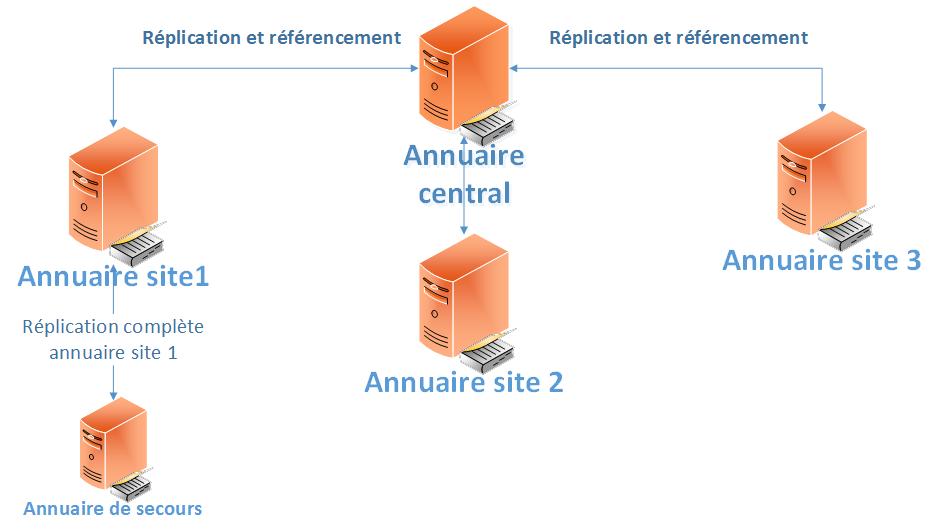
\includegraphics[scale=0.6]{Images/SchemaGlobal.png}
	\caption{Architecture globale}
	\label{SchemaGlobal}
\end{figure}
L’annuaire global, situé au siège du la société, rassemble toutes les informations et les annuaires locaux ne contiennent que les informations sur les utilisateurs présents sur chaque site. Ainsi, des mécanismes de référencement et de réplication entre les serveurs locaux et le serveur central pourront être mis en place.
De plus, un serveur de secours pourra assurer une haute disponibilité de l’annuaire local avec une réplication périodique des données de ce dernier.
\chapter{Quand s'authentifier ?}
Tout d’abord, il est nécessaire de définir le cadre dans lequel le module sera utilisé : un utilisateur pourra effectuer toutes les modifications sur sa base de données interne, ce n’est que lors de la synchronisation des données que l’utilisateur devra s’authentifier.

L’authentification permettra de déterminer quelles sont les modifications que l’utilisateur a le droit d’apporter à la base de données. Ainsi, aucun annuaire ne sera installé sur les postes clients, évitant toute tentative frauduleuse d’accorder des droits différents à une personne.
\begin{figure}[htbp]
	\centering
	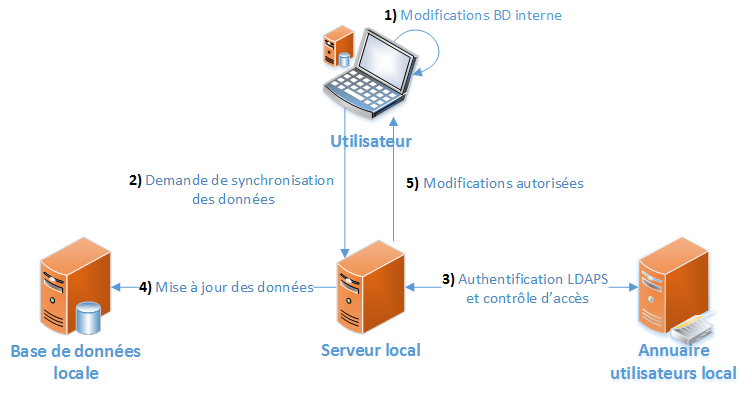
\includegraphics[scale=0.9]{Images/SchemaAuthentification.png}
	\caption{Authentification pour la synchronisation}
	\label{SchemaAuthentification}
\end{figure}

Les serveurs mis en place prennent en charge le protocole non standard « LDAPS » (LDAP over SSL). Ce protocole utilise le port 10636 (ou 636). Le protocole LDAPS diffère du LDAP sur deux points :
\begin{itemize}
\item à la connexion, le client et le serveur établissent une connexion TLS avant que n'importe quelle autre commande LDAP ne soit envoyée,
\item la connexion LDAPS doit être fermée lors de la clôture de TL
\end{itemize}

Ce protocole permet de ne pas faire transiter les mots de passe en clair sur le réseau et ainsi garantir leur confidentialité.
\chapter{Droits utilisateurs}
Les droits des utilisateurs sont stockés dans des attributs LDAP ajoutés aux informations standards. Chaque utilisateur dispose de droits qui lui sont propres, mais aussi de droits liés au(x) groupe(s) auquel(s) il appartient.
Voici la liste des champs créés pour définir les droits d’une personne :
\begin{itemize}
\item aFieldRead : Autorisation de lecture d’un champ d’une table
\item aFieldWrite : Autorisation d’écriture d’un champ d’une table
\item aTableAdd : Autorisation d’ajout d’une ligne d’une table
\item aTableDel : Autorisation en suppression d’une ligne d’une table
\item rFieldRead : Refus en lecture d’un champ d’une table
\item rFieldWrite : Refus en écriture d’un champ d’une table
\item rTableAdd : Refus d’ajout d’une ligne d’une table
\item rTableDel : Refus en suppression d’une ligne d’une table
\end{itemize}

Ces attributs permettent de definir soit l'ensemble des permissions, soit l'ensemble des refus  : si un attribut autorise la lecture pour un champ cela implique que la lecture des autres champs sera interdite.

Ci-dessous deux exemples d’attribut et leur valeurs :
\begin{itemize}
\item Autorisation lecture des champs RequisitionID, VehicleID et TransportMean table Waybill : 
aFieldRead : Waybill(RequisitionID, VehicleID, TransportMean)
\item Refus d’ajout d’un champ dans la table Requisition : 
rTableAdd : Requisition
\end{itemize}

On remarque pour le premier exemple qu’il ne sera pas nécessaire de remplir le champ rFieldRead pour la table Waybill car il est sous-entendu que l’accès en lecture aux autres champs de la table Waybill sera refusé. 

\chapter{Réalisation}

Il a été demandé par l’équipe chargée de la synchronisation de fournir des méthodes permettant de savoir, pour un utilisateur donné, s’il a le droit d’ajouter/supprimer dans telle table ou telle table, ou de lire/écrire tel champ ou tel champ dans une table. 

Pour ce faire, nous avons implementé un module sous c++/Qt selon le PAQ en utilisant les librairies LDAP trouvable à cette adresse http://www.novell.com/developer/ndk/ldap\_libraries\_for\_c.html.

\section{Annuaire ldap}
L'installation du serveur ldap est faite sous le système windows 7/32 bits ( système utilisé actuellement selon le cahier des charges de consultation), mais aussi sous le système Linux ce qui est demandé pour une imigration future. 

\section{Gestion des conflits}
\begin{figure}[htbp]
	\centering
	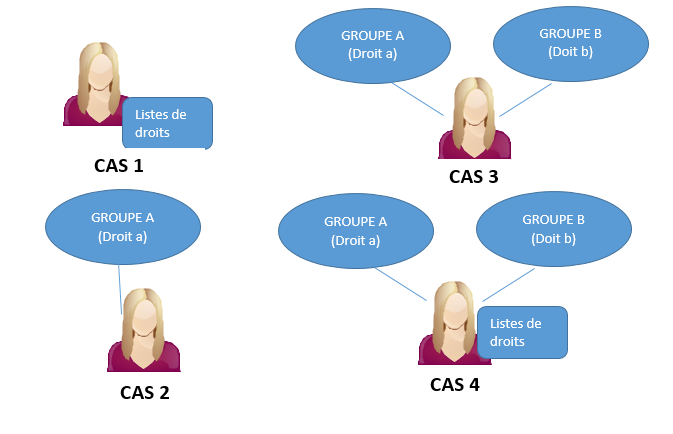
\includegraphics[scale=0.7]{Images/conflitsDroits.png}
	\caption{Quelques exemples de demande de permission }
	\label{conflitsDroits}
\end{figure}

Voici comment fonctionne notre outil lors des différents demandes des permissions
\begin{itemize}
\item \textbf{CAS 1 } : L'utilisateur aura directement ses permissions
\item \textbf{CAS 2 } : L'utilisateur aura les permissions du groupe
\item \textbf{CAS 3 } : Priorité aux permissions autorisées entre les groupes
\item \textbf{CAS 4 } : Priorité aux permissions directement liées à l'utilisateur
\end{itemize}

\chapter{Déploiement}
\section{Serveurs}
\subsection{Windows}
La technologie utilisée pour la mise en place des serveurs d’annuaires est Apache DS. Afin de mettre en place le serveur sur une machine Windows, télécharger et installer le logiciel Apache DS à l’adresse suivante http://directory.apache.org/apacheds/ (ou bien chercher ApacheDS sur votre moteur de recherche préféré). Suite à l’installation, le service ApacheDS - default est démarré, le serveur écoute maintenant sur les ports 10389 et 10636.

Afin de configurer et gérer le serveur il est possible d’installer le logiciel Apache Directory Studio qui fournir une interface utilisateur simple et ergonomique. Pour cela il suffit de créer une connexion sur le serveur via son adresse et le port d’écoute.

Pour générer l’annuaire que nous avons conçu, créer une partition nommée GarmirKatch dont le suffixe sera dc=GarmirKatch,dc=fr. Importer via Apache Directory Studio les fichiers schemagarmirApache.ldif, Racine.ldif, Users.ldif, Groups.ldif et Missions.ldif dans le serveur.
\subsection{Linux}
Pour configurer votre serveur linux voir cette adresse\footnote{http://www.bgeek-france.ec0.fr/2011/10/23/admin/linux/installation-et-parametrage-de-\%C2\%AB-base-\%C2\%BB-d\%E2\%80\%99openldap-ubuntu-11-04-et-ubuntu-11-10-mode-cnconfig.html }
, vous y trouverez toutes les explications pour installer et configurer votre serveur.

Toute fois, ci joint à documentation les fichiers Database.ldif, GarmirShema.ldif, Racine.ldif, Users.ldif, Groups.ldif et Missions.ldif qui sont des fichiers de configurations.
\section{Configuration des clients}
Chaque client devra être configuré avant de partir en mission pour intégrer l’adresse et le port d’écoute du serveur. 

\chapter{Livrables}
L’intégration du module dans l’application se fait grâce aux livrables fournis aux parties prenantes de l’application (ici l’équipe chargée de la synchronisation des données) :
\begin{itemize}
\item Les librairies et les sources du module ( windows/32 bits, linux)
\item Une documentation d’utilisation des classes C++
\end{itemize}
\end{document}